\section{Current Status and Characteristics (RQ1)}

\subsection{RQ1.1 How Frequently Do Different Large Language Models Generate Hallucinated Packages in Real Development Scenarios, and What Are the Distribution Characteristics of the Generated Packages? Are There Significant Differences Across Models?}

\begin{figure}[t]
\centering
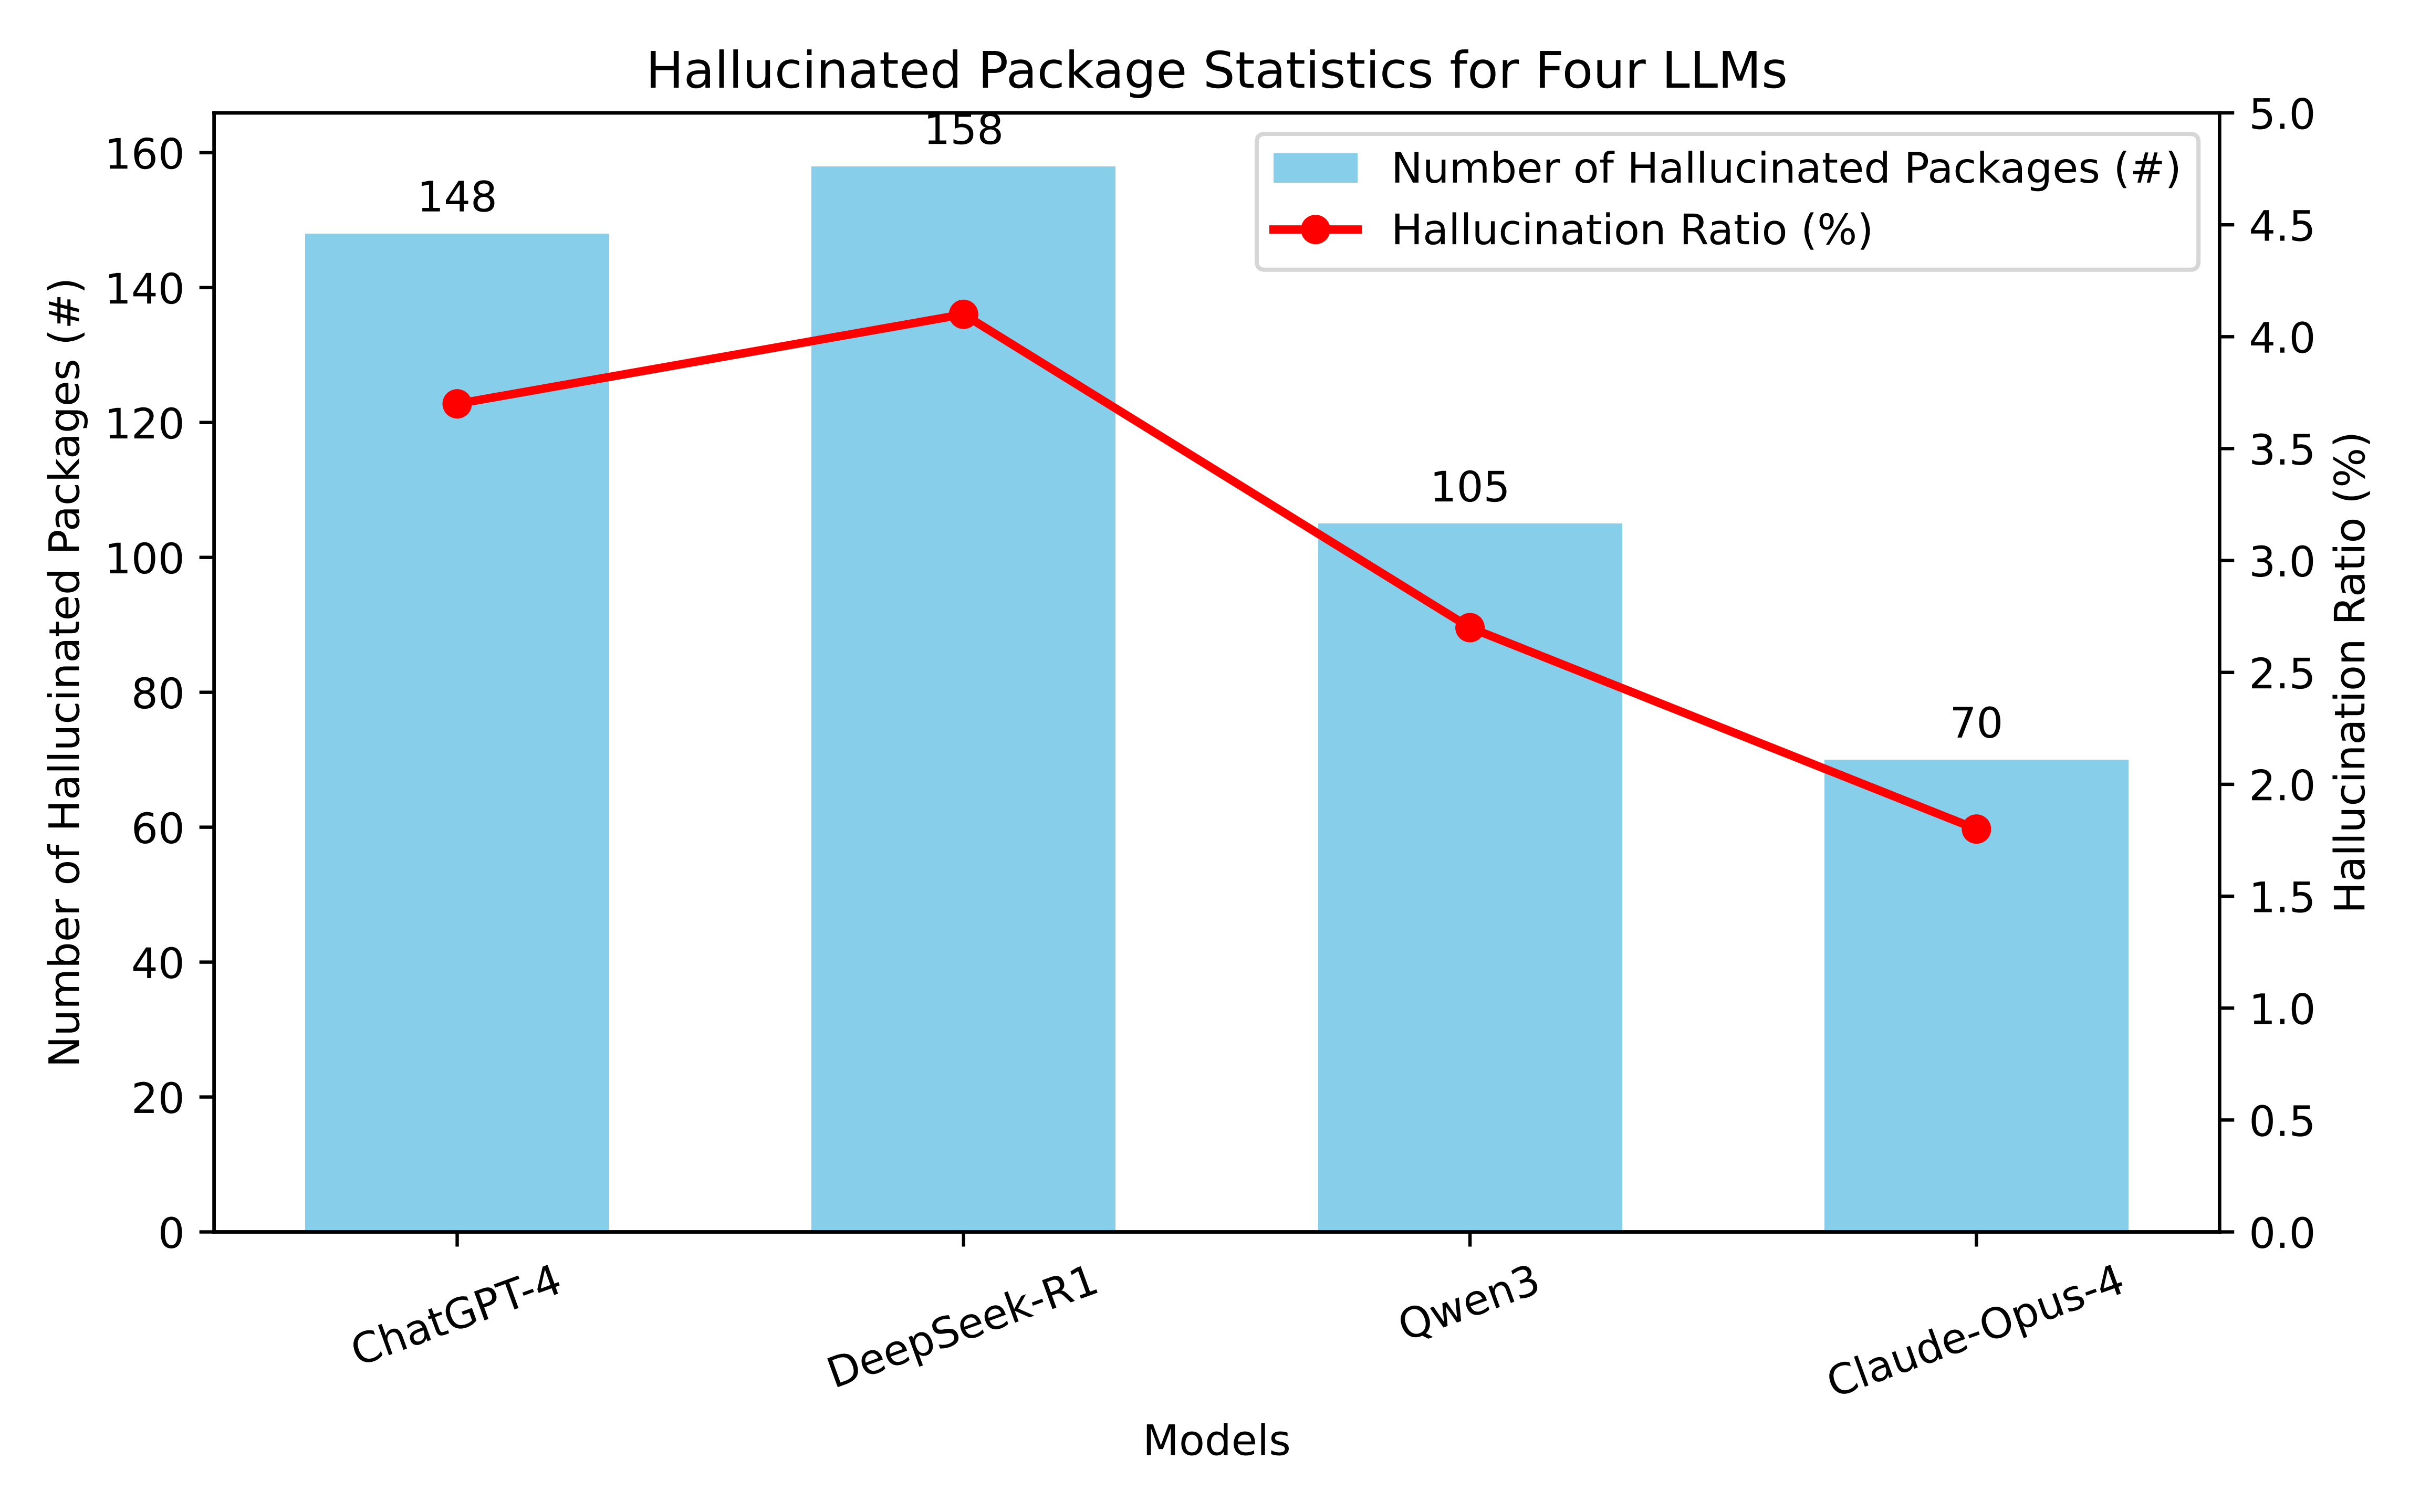
\includegraphics[width=0.9\linewidth]{fig/RQ1.1-hallucinated-frequency.png}
\caption{Number and Ratio of Hallucinated Packages Generated by Different Large Language Models}
\label{fig:rq1-1-hallucinated-frequency}
\end{figure}


To compare the frequency and potential risk of hallucinated package generation by different large language models in real development scenarios, we counted the number 
of hallucinated packages generated by four models on the functional question dataset, as well as their corresponding proportions, as shown in 
Fig.~\ref{fig:rq1-1-hallucinated-frequency}. It should be noted that this study focuses on the potential misleading risk that models may pose to 
developers when recommending software packages in practice. Therefore, when calculating the hallucination ratio, we used the number of questions for which the 
model explicitly recommended at least one package name as the denominator, and excluded questions where the model returned \textit{no\_package}. This is because 
in such cases the model did not perform any package recommendation and thus would not directly affect developers.

From the statistical results, it can be observed that all evaluated large language models generate hallucinated packages for a certain proportion of questions, 
indicating that this phenomenon is common across different models. On this basis, different models exhibit relatively significant differences in both the number 
and the proportion of hallucinated packages generated. Among them, DeepSeek-R1 generates the largest number of hallucinated packages and also has the highest 
hallucination ratio, reaching 4.02\%; ChatGPT-4 ranks second, while Qwen3 and Claude-Opus-4 generate relatively fewer hallucinated packages. However, even for 
Claude-Opus-4, which has the lowest hallucination ratio among the evaluated models, the ratio still reaches 1.72\%, indicating that hallucinated packages are not 
caused by a few individual models or extreme cases, but rather represent a potential risk that commonly exists when large language models perform software package 
recommendation tasks.

\begin{figure}[t]
\centering
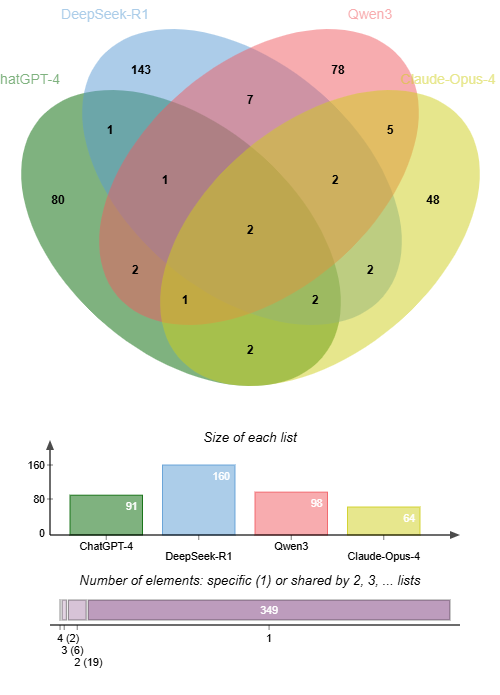
\includegraphics[width=0.9\linewidth]{fig/RQ1.1-hallucinated-overlap.png}
\caption{Intersection and Union Distribution of Hallucinated Packages Generated by Different Large Language Models}
\label{fig:rq1-1-hallucinated-overlap}
\end{figure}

After analyzing the frequency of hallucinated packages generated by different large language models, we further examined the consistency relationships among the 
hallucinated packages generated by these models. Specifically, we compared the sets of hallucinated packages generated by the four models and conducted an 
intersection–union analysis to examine whether there exist hallucinated packages that are simultaneously generated by multiple models, as shown 
in Fig.~\ref{fig:rq1-1-hallucinated-overlap}.

The results show that the vast majority of hallucinated packages are generated by only a single model, and the overall overlap among different models is relatively 
low. Only a very small number of hallucinated packages are recommended simultaneously by two or more models. This result indicates that the generation of hallucinated 
packages does not mainly originate from a few “highly misleading” fixed package names, but is more likely related to the randomness during the generation process, 
inference biases, or differences in contextual understanding across models. Therefore, the generation behavior of hallucinated packages exhibits strong model-specific 
characteristics across different models.

\begin{figure}[t]
\centering
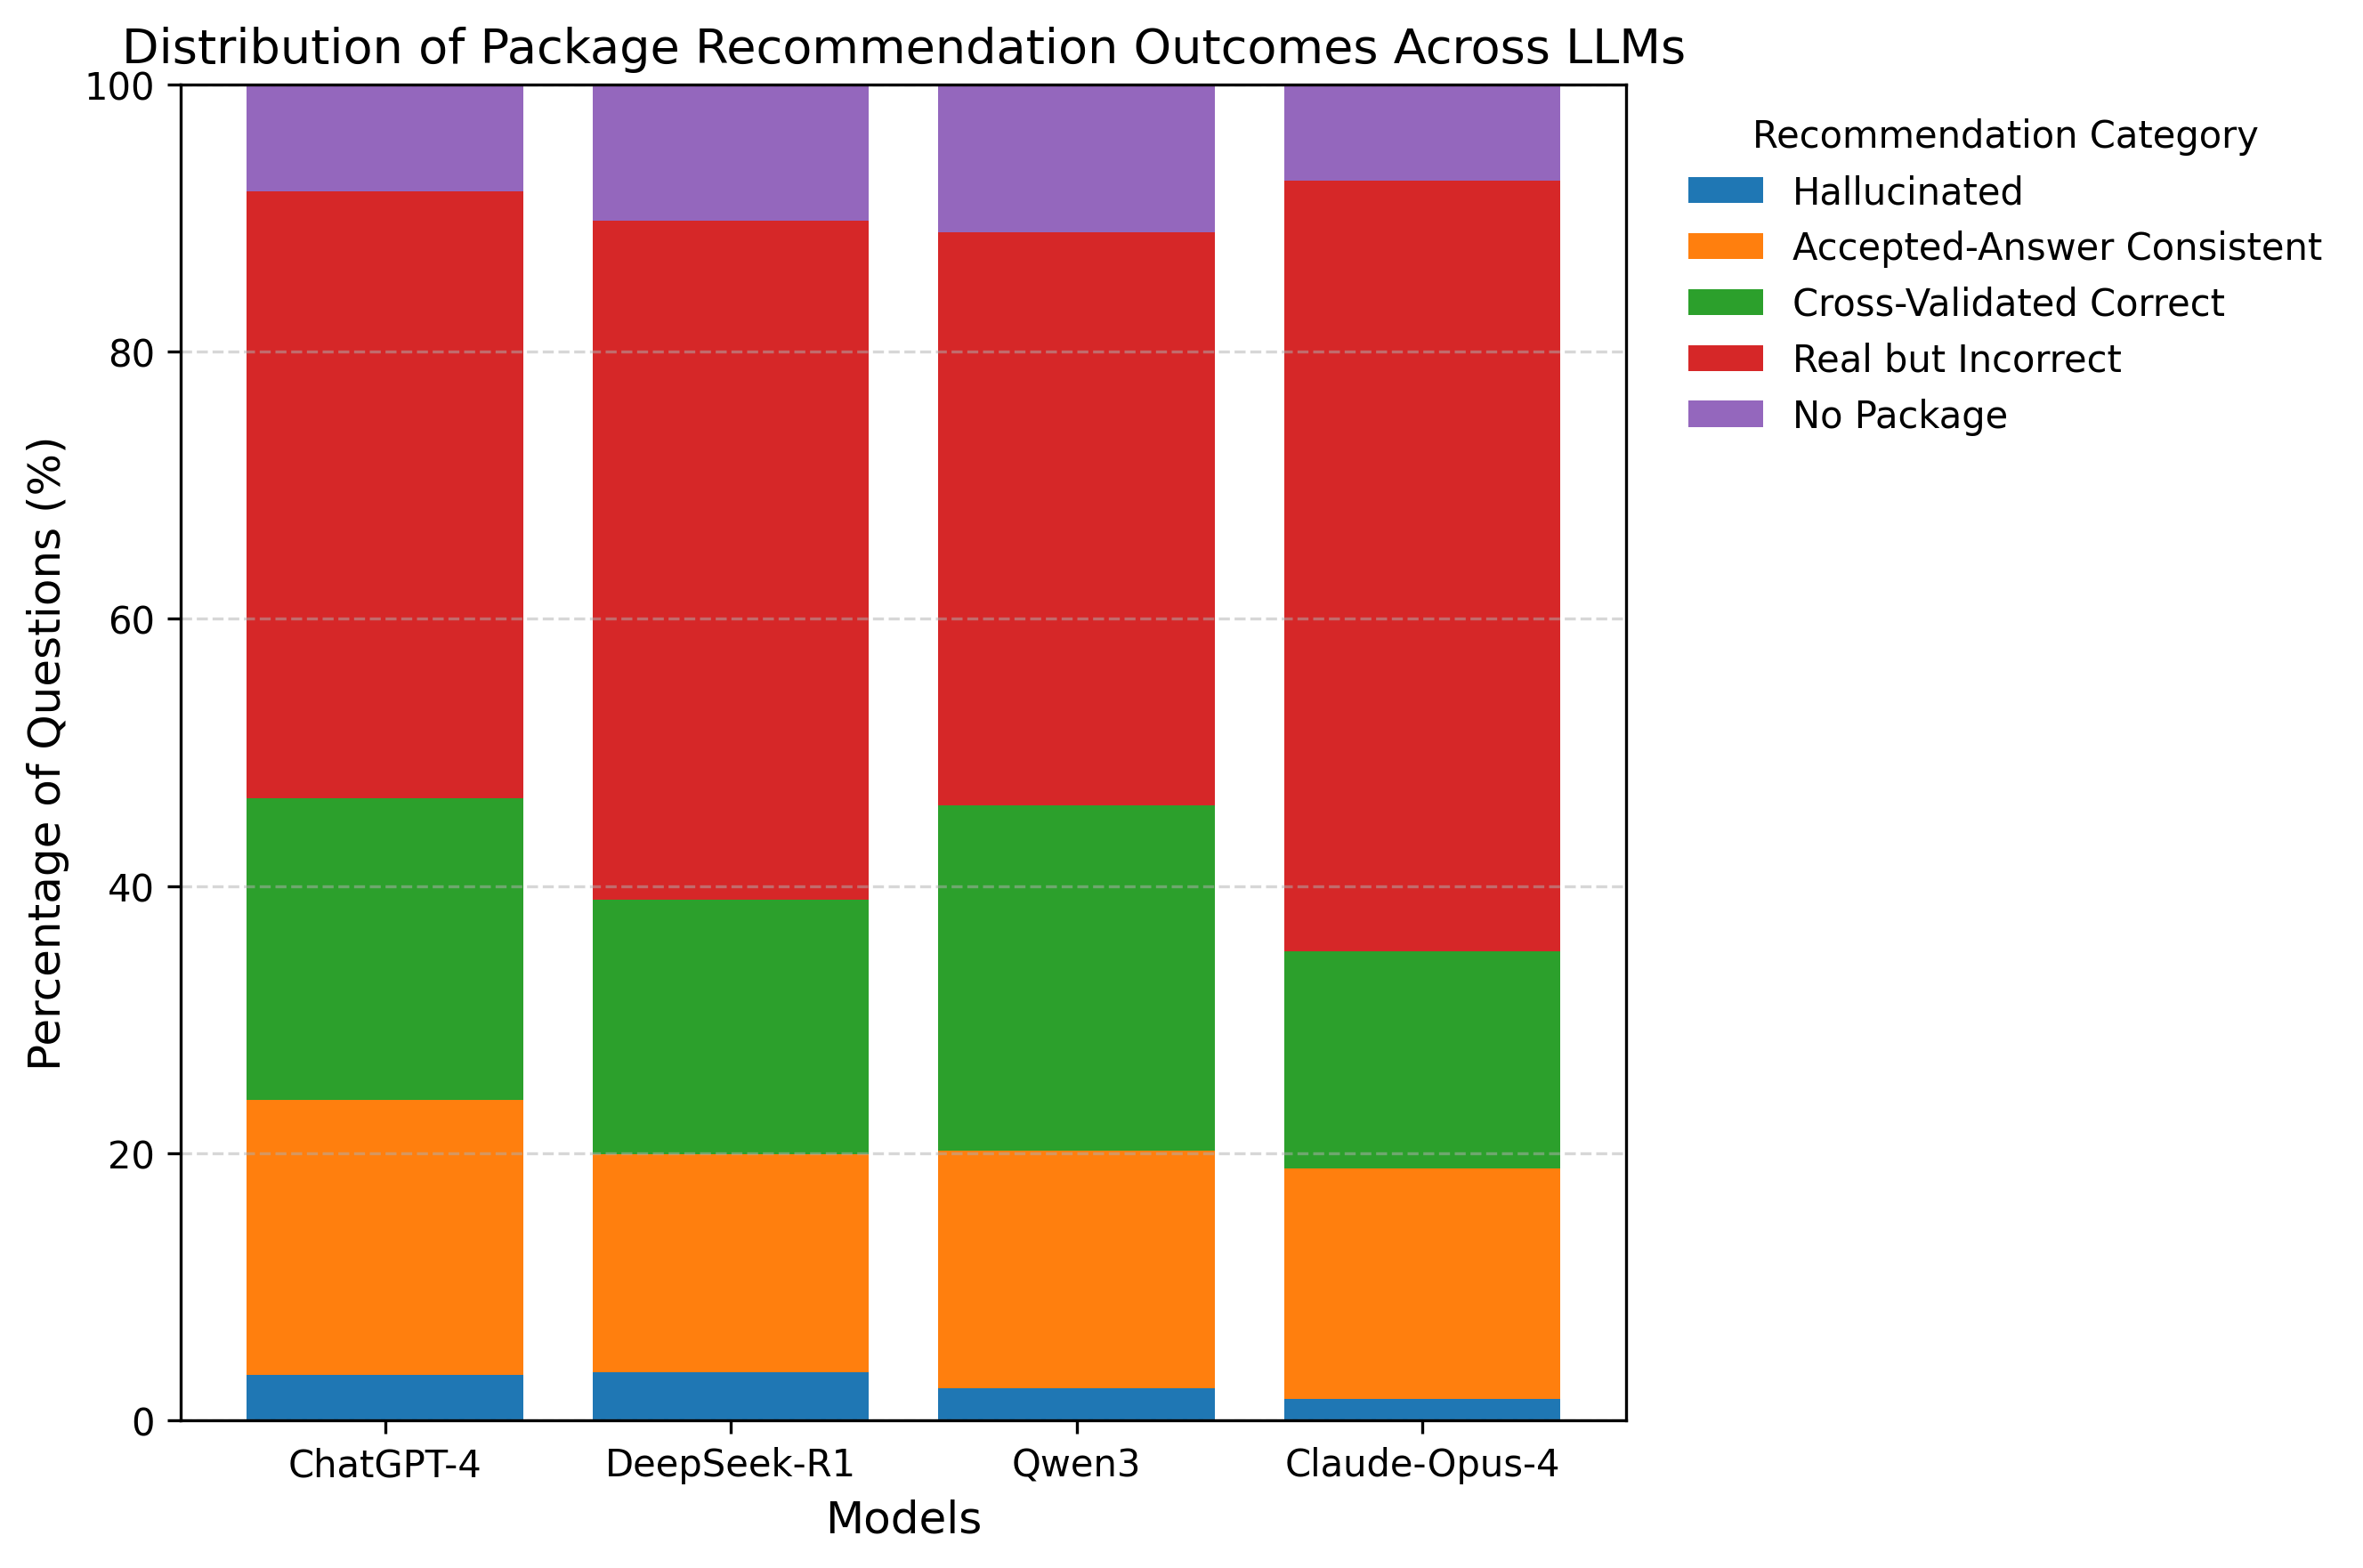
\includegraphics[width=0.9\linewidth]{fig/RQ1.1-recommendation-distribution.png}
\caption{Category Distribution of Package Recommendation Outcomes Across Different Large Language Models}
\label{fig:rq1-1-recommendation-distribution}
\end{figure}

Existing studies that analyze the problem of hallucinated packages recommended by large language models often mainly focus on the proportion of hallucinated packages 
generated. However, examining the issue solely from the single perspective of hallucinated packages is insufficient to comprehensively characterize the overall 
behavioral patterns of models in software package recommendation tasks. In addition to hallucinated packages, whether the packages recommended by a model are consistent 
with the real solutions, or at least correspond to reasonable and usable third-party packages, is also an important aspect for understanding its recommendation 
behavior, and helps us analyze the underlying mechanisms of hallucinated package generation from a more comprehensive perspective. Based on this consideration, we 
further analyze the distribution of recommendation outcomes of different large language models in package recommendation tasks from an overall perspective.

Specifically, for each question, we denote the set of third-party software packages used in the accepted answer as $A$, which we regard as the set of packages adopted 
by the correct solution for that question in real development scenarios. We denote the set of high-confidence correct packages obtained through cross-validation across 
multiple models as $C$, where each package must satisfy two conditions: it is consistently recommended by at least three different large language models and is 
verified by PyPI to be a real existing package rather than a hallucinated one. We denote the set of packages actually recommended by the model as $P$, among which 
the subset identified as hallucinated packages is denoted as $H$. Based on these definitions, for each question we categorize the model’s recommendation outcome into 
the following five cases:

(1) \textbf{Hallucinated}: when $H \neq \varnothing$, the model generates at least one hallucinated package;

(2) \textbf{Accepted-Answer Consistent}: when $P \subseteq A$, the packages recommended by the model are completely consistent with the packages used in the accepted answer;

(3) \textbf{Cross-Validated Correct}: when $P \subseteq A \cup C \;\wedge\; P \nsubseteq A$, the packages recommended by the model do not all appear in the accepted answer, but are supported by cross-validation across multiple models;

(4) \textbf{Real but Incorrect}: when all packages in $P$ are real packages, but at least one package does not belong to $A \cup C$;

(5) \textbf{No Package}: the model returns \textit{no\_package}, meaning that the model does not provide any third-party package recommendation.

Based on the above classification rules, we calculated the proportional distribution of the five categories of package recommendation outcomes for the four large 
language models, as shown in Fig.~\ref{fig:rq1-1-recommendation-distribution}. From the overall results, \textit{Real but Incorrect} occupies the highest proportion 
across all models, and its proportion is overall higher than the combined proportion of the two correct recommendation categories, \textit{Accepted-Answer Consistent} 
and \textit{Cross-Validated Correct}. This indicates that, compared with completely fabricated package names that do not exist, a more common error form in package 
recommendation tasks is that models recommend packages that actually exist but are not suitable for the current problem. This type of error occupies the main 
proportion in the overall recommendation behavior.Meanwhile, all four models return \textit{no\_package} for a certain proportion of questions. This phenomenon 
indicates that when the model cannot determine an appropriate third-party package, it does not always forcibly provide a recommendation, but instead demonstrates a 
certain degree of conservativeness in its responses, which can to some extent avoid arbitrary guessing. This reflects a trade-off between ``recommendation 
activeness'' and ``answer cautiousness'' in software package recommendation tasks.In addition, although the proportion of \textit{Hallucinated} in the overall 
distribution is relatively small, it still appears across all models. Moreover, its potential harm differs from other error types, as it may cause additional 
debugging costs for developers and even introduce risks to the software supply chain. Therefore, it still has non-negligible research significance.

Beyond the overall distribution characteristics, the proportions of the five recommendation outcome categories also exhibit noticeable differences across different 
models, reflecting different tendencies in package recommendation strategies among models. On the one hand, the proportions of \textit{No Package} 
and \textit{Real but Incorrect} differ across models: some models choose to return \textit{no\_package} for a larger number of questions, demonstrating a more 
conservative recommendation tendency; whereas other models tend to provide specific package recommendations, which also to some extent increases the proportion 
of recommending real but unsuitable packages.On the other hand, differences also exist in the overall proportions between recommending correct packages and 
incorrect packages across models. Some models have higher proportions in the two categories \textit{Accepted-Answer Consistent} and \textit{Cross-Validated Correct} 
compared with other models, indicating that they are overall more likely to recommend correct packages. In contrast, other models relatively more frequently 
recommend packages in the \textit{Real but Incorrect} and \textit{Hallucinated} categories, indicating that they are more likely to produce inappropriate 
recommendations in package recommendation tasks.These differences indicate that under the same question set and unified prompting conditions, the overall 
reliability levels of different large language models in software package recommendation tasks are not consistent.

Based on the above analyses, we can draw the following conclusion: different large language models inevitably generate a certain proportion of hallucinated 
packages in software package recommendation tasks under real development scenarios, indicating that this phenomenon has a certain degree of universality. Meanwhile, 
further intersection–union analysis shows that hallucinated packages are mostly model-specific rather than concentrated in a few fixed package name patterns. 
In addition, from the perspective of the overall recommendation outcomes, large language models are more likely to recommend packages that do not match the 
requirements of the current problem in software package recommendation tasks (including both hallucinated packages and real packages that are not suitable for 
the current problem), which reflects a certain degree of reliability deficiency in their recommendation decision process.

\subsection{RQ1.2 What Patterns Can Be Observed in the Naming Structures, Semantic Sources, and Domain Distributions of Hallucinated Packages Generated by Large Language Models?}

\subsection{RQ1.3 Do Questions That Lead to Hallucinated Packages Exhibit Specific Semantic Characteristics? Which Types of Questions Are More Likely to Trigger Hallucinated Packages?}

In the previous sections, we mainly analyzed the phenomenon of hallucinated packages, including the frequency of hallucinated package generation, the differences 
across different models, and the overall distribution characteristics of package recommendation outcomes. We further examined the naming structures, semantic 
sources, and domain distribution patterns of hallucinated packages. However, examining the issue solely from the perspectives of model outputs and the hallucinated 
packages themselves is still insufficient to fully explain the underlying causes of hallucinated package generation. Whether the questions that lead to 
hallucinated packages themselves possess potential characteristics is also worth investigating. Therefore, in this subsection we analyze whether the questions 
that produce hallucinated packages exhibit certain specific characteristics that make large language models more likely to generate hallucinations on these questions.

To answer this question, we first counted the number of times that each question triggered hallucinated package recommendations across the four large language models 
(ChatGPT-4, DeepSeek-R1, Qwen3, and Claude-Opus-4), and used this count as an indicator to measure the hallucination degree of each question. This indicator 
reflects whether different models exhibit consistent tendencies to generate hallucinated packages when facing the same question. Based on this statistical result, 
we categorized the questions into different groups according to the number of large language models that triggered hallucinated packages for each question, 
denoted as $H$.

In this dataset, the numbers of questions in the four groups with $H = 0$, $H = 1$, $H = 2$, and $H = 3$ are 3979, 333, 62, and 8, respectively. It should be 
noted that among all questions, there is no case in which hallucinated packages are recommended simultaneously by all four large language models. Based on the 
above grouping method, we conduct a systematic analysis of the potential differences in how different questions trigger hallucinated packages from three aspects: 
input complexity of the questions, global semantic structure, and local semantic neighborhood structure.

\begin{table}[t]
\centering
\caption{Statistics of Input Complexity and Local Semantic Features for Questions with Different Hallucination Intensities}
\label{tab:rq1-3-input-complexity}
\begin{tabular}{c c c c c c}
\toprule
Hallucination Count ($H$) & Question Count & Avg. Token Count & Median Token Count & Neighbor Hallucination (Mean) & Neighbor Hallucination (Median) \\
\midrule
0 & 3979 & 12.278 & 12.000 & 0.0853 & 0.05 \\
1 & 333 & 11.733 & 11.000 & 0.161 & 0.1 \\
2 & 62 & 11.984 & 11.500 & 0.2137 & 0.2 \\
3 & 8 & 13.625 & 12.500 & 0.1625 & 0.15 \\
\bottomrule
\end{tabular}
\end{table}

\subsubsection{Input Complexity Analysis}

Based on the above grouping, we first examine whether the input complexity of questions is related to the generation of hallucinated packages. Considering 
that large language models process inputs using tokens rather than character counts during actual inference, this study adopts the \textit{tiktoken} tool 
provided by OpenAI to tokenize each question and calculate the corresponding number of tokens, which is used as the metric for measuring the input complexity 
of questions.

On this basis, we further analyzed the distribution of token counts across questions with different hallucination intensities. Table~\ref{tab:rq1-3-input-complexity} 
summarizes the number of questions in each hallucination intensity group, along with the corresponding average token counts and median token counts. From the overall 
results, the input complexity across different hallucination intensity groups does not exhibit an obvious monotonic pattern, and the differences among the groups 
are overall relatively limited.

To further examine whether the differences in input complexity among questions with different hallucination intensities are statistically significant, we employed 
the Kruskal--Wallis nonparametric test to compare the token count distributions across the four groups of questions. The test results show that the differences in 
token counts among the hallucination intensity groups do not reach statistical significance ($p = 0.052$).

This result indicates that, within the dataset used in this study, there is insufficient evidence to conclude that the input complexity of a question significantly 
affects the likelihood of large language models generating hallucinated packages. From this perspective, the occurrence of hallucinated packages cannot be simply 
attributed to increases in question length or the amount of input information. Instead, whether a question triggers hallucinated packages may be more closely 
related to its semantic expression patterns and deeper semantic structural characteristics. Therefore, in the subsequent analysis, we further investigate the 
questions from the perspective of semantic structure.

\subsubsection{Global Semantic Structure Analysis}

\begin{figure}[t]
\centering
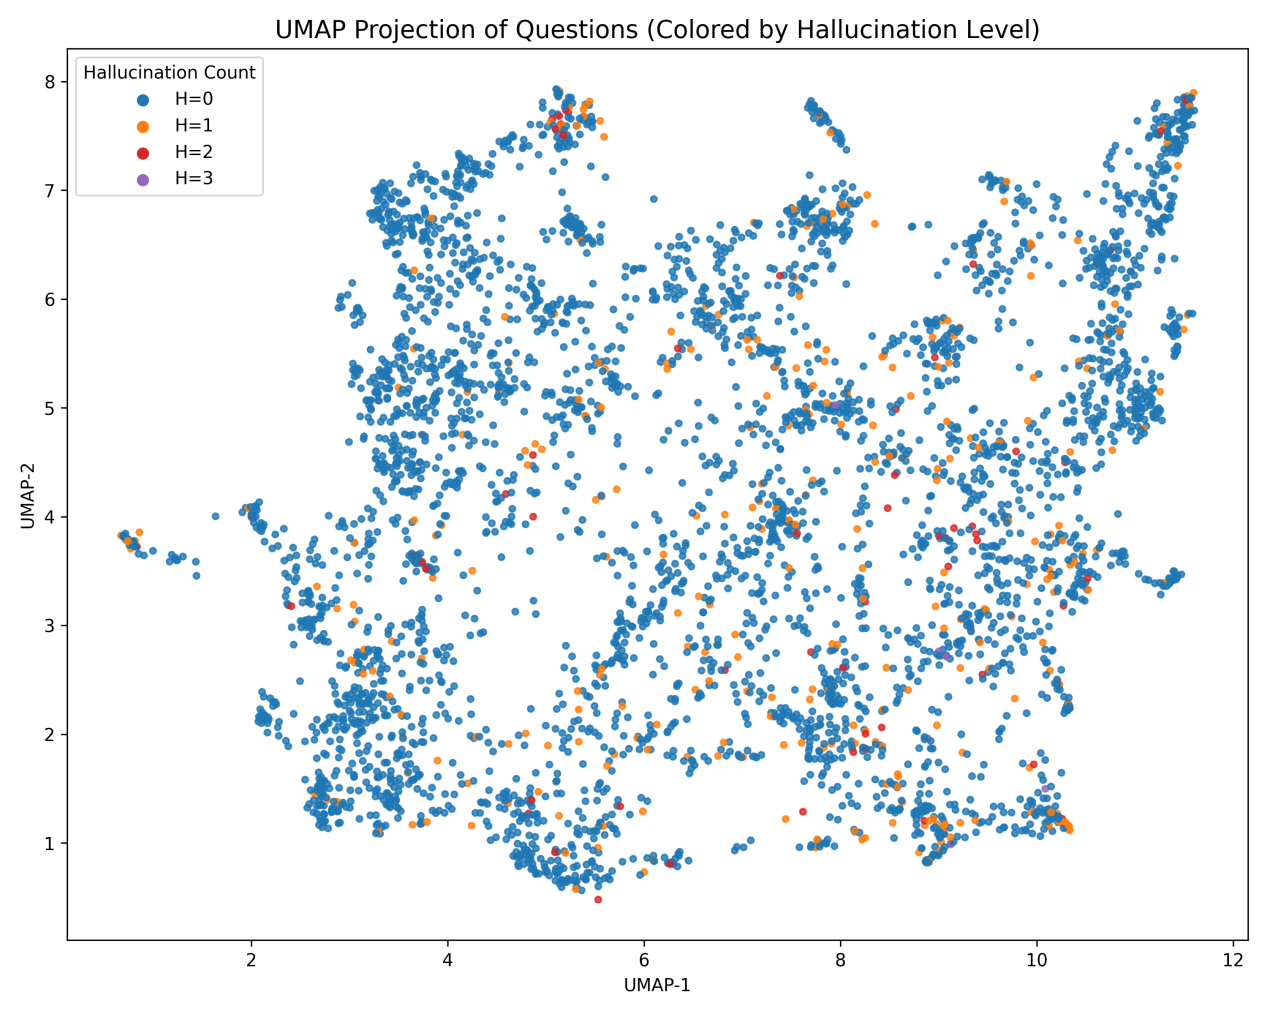
\includegraphics[width=0.95\linewidth]{fig/RQ1.3-umap.png}
\caption{UMAP Visualization of Questions in the Semantic Space Colored by Hallucination Intensity}
\label{fig:rq1-3-umap}
\end{figure}

In the previous subsection, we found that the input complexity of questions cannot sufficiently explain the differences in the generation of hallucinated packages. 
Based on this finding, we further examine the distribution of questions with different hallucination intensities in the semantic space from the perspective of 
global semantic structure, in order to analyze whether the occurrence of hallucinated packages is related to the semantic topics or broader semantic regions 
to which the questions belong.

Specifically, we employ the Sentence-BERT model \textit{all-mpnet-base-v2} to generate sentence embeddings for each question, thereby capturing the semantic 
characteristics of the questions in a high-dimensional semantic space. Subsequently, we apply the UMAP method to reduce the dimensionality of the high-dimensional 
semantic vectors and project them into a two-dimensional space for visualization. During the visualization process, questions are color-coded according to the 
number of large language models that generated hallucinated packages for each question ($H$), allowing us to observe the distribution differences of questions 
with different hallucination intensities in the global semantic space.

Figure~\ref{fig:rq1-3-umap} presents the projection of questions with different hallucination intensities in the UMAP semantic space. From the overall distribution, 
the questions form several continuous and dense regions in the semantic space. However, questions with different hallucination intensities do not form clearly 
separable clusters or boundaries within these semantic regions. Questions that trigger hallucinated packages ($H \geq 1$) are highly intermixed with those that 
do not trigger hallucinated packages ($H = 0$), and they do not appear to concentrate in any specific semantic region or topic cluster.

This result indicates that the occurrence of hallucinated packages is not concentrated within a small number of specific semantic topics or question types. 
In other words, from the perspective of global semantic distribution, questions that trigger hallucinated packages do not exhibit a clear “topic bias” or 
“domain concentration.” Instead, the hallucinated package phenomenon is more likely to be a behavior that occurs broadly across different semantic regions, 
rather than being systematically triggered by certain specific semantic topics.

\subsubsection{Local Semantic Neighborhood Structure Analysis}

In the preceding analyses, we found that neither the input complexity of questions nor their positions in the global semantic space are sufficient to explain 
the differences in hallucinated package generation. Based on this observation, we further investigate the phenomenon from the perspective of local semantic 
structure, examining whether the generation of hallucinated packages exhibits potential correlations within neighborhoods of semantically highly similar questions.

Specifically, we use the Sentence-BERT model \textit{all-mpnet-base-v2} to generate sentence embeddings for each question, in order to capture the semantic 
characteristics of questions in the high-dimensional semantic space. Subsequently, for each question in the dataset, we retrieve the 20 most semantically 
similar questions in the embedding space based on cosine similarity. The average number of large language models that generate hallucinated packages among these 
semantically similar questions is then used as the neighborhood hallucination value for the given question. This metric characterizes the overall degree to 
which the hallucinated package phenomenon occurs within the set of questions that are highly similar to a given question in semantic space.

Based on this, we further group the questions according to the number of large language models that generate hallucinated packages for each question ($H$), 
and analyze the distribution of neighborhood hallucination values across different hallucination intensity groups. The statistical results are summarized in 
Table~\ref{tab:rq1-3-input-complexity}. From Table~\ref{tab:rq1-3-input-complexity}, it can be observed that questions that trigger hallucinated 
packages ($H \geq 1$) and those that do not trigger hallucinated packages ($H = 0$) exhibit relatively clear differences in their neighborhood hallucination 
values. Specifically, questions that do not trigger hallucinated packages ($H = 0$) have the lowest neighborhood hallucination values, whereas the $H = 2$ group 
shows the highest average level of neighborhood hallucination.

To further examine whether the differences in neighborhood hallucination values among questions with different hallucination intensities are statistically 
significant, we employ the Kruskal--Wallis nonparametric test to compare the four groups of questions. The test results indicate that the differences in the 
average neighborhood hallucination values among the groups are highly statistically significant ($p < 0.001$).

This result indicates that the generation of hallucinated packages is neither entirely random nor an occasional phenomenon independent of the semantic structure 
of questions. Although questions that trigger hallucinated packages do not exhibit clear topic-level clustering in the global semantic space, the hallucinated 
package phenomenon shows a significant degree of consistency within local neighborhoods of semantically similar questions. This suggests that hallucinated 
packages are more likely related to the expression patterns or implicit semantic details of questions at the local semantic level. It should be noted that 
we do not further investigate these specific semantic factors; rather, through empirical analysis we reveal the existence of such local correlations. 
A deeper investigation into the underlying semantic mechanisms behind this phenomenon remains a promising direction for future research.